\section{Рабочий проект}
\subsection{Спецификация компонентов и классов системы}
\subsubsection{Спецификация пользовательской части системы}
Главная страница системы
Предоставляет точку входа в приложение, отображает маркетинговую информацию, преимущества компании и примеры работ. Служит навигационным хабом для перехода к ключевым функциям системы.

Взаимодействия:
\begin{itemize}
	\item Связь с order\_form.php;
	\item интеграция с edit\_content.php для административного доступа;
	\item использование logout.php для смены учетной записи.
\end{itemize}

Использует CSS Grid и медиазапросы для перестроения макета на мобильных устройствах.
Горизонтальная карусель с hover-эффектами на изображениях.

Зависимости:
\begin{itemize}
\item внешний CSS-файл: style.css;
\item локальные изображения: images/pc\_build1-5.jpg;
\item поддержка PHP для обработки даты.
\end{itemize}

Спецификация компонента: order\_form.php
Система оформления заказов
Обрабатывает создание заказов на сборку компьютеров. Управляет выбором компонентов, валидацией данных и транзакционным обновлением остатков на складе.

Взаимодействия:
\begin{itemize}
	\item интеграция с MySQL БД;
	\item связь с index.php и edit\_content.php через навигацию;
	\item использование logout.php для смены пользователя.
\end{itemize}

Безопасность и валидация:
Осуществляется через подготовленные SQL-запросы (prepare + bind\_param), экранирование вывода (htmlspecialchars).

Валидация ввода: 
Проверяется формат цены, должна быть числом и ограничение по размеру, контролирует даты, предотвращает ввод некорректного формата данных с помощью выпадающего календаря и проверяет даты на корректный ввод, каждый компонент предлагается из SQL, проверяется его наличие и существование.

\renewcommand{\arraystretch}{0.8}
\begin{xltabular}{\textwidth}{|p{4.5cm}|>{\setlength{\baselineskip}{0.7\baselineskip}}p{5.5cm}|>{\setlength{\baselineskip}{0.7\baselineskip}}p{5.5cm}|}
	\caption{Описание функций и скриптов, используемых в приложении\label{class:table}}\\
	\hline \centrow Название компонента & \centrow Описание & \centrow Методы / Действия \\
	\hline \endfirsthead
	\caption*{Продолжение таблицы \ref{class:table}}\\
	\hline \centrow Название компонента & \centrow Описание & \centrow Методы / Действия \\
	\hline \endhead
	
	getComponents & Получает массив данных из таблицы БД (комплектующие, клиенты, мастера) & Формирует и выполняет SELECT-запрос, возвращает ассоциативный массив \\\hline
	
	get\_id\_column & Возвращает имя id-столбца для таблицы комплектующих & Сопоставляет название таблицы с её id-столбцом \\\hline
	
	get\_table\_name & Возвращает имя таблицы по имени id-поля & Сопоставляет поле с таблицей, возвращает строку \\\hline
	
	toggleDropdown & Переключает видимость выпадающего списка (dropdown) & Находит список по id, переключает класс show, фокусирует input \\\hline
	
	showDropdown & Показывает нужный выпадающий список & Скрывает все списки, затем показывает нужный (добавляет класс show) \\\hline
	
	filterDropdown & Фильтрует элементы списка по введённому тексту & Сравнивает текст каждого li с введённым значением, скрывает/показывает элементы \\\hline
	
\end{xltabular}
\renewcommand{\arraystretch}{1.0}

\newpage
\subsubsection{Спецификация панели администратора}
Основная страница (edit\_content.php)
Центральный интерфейс управления данными системы. Предоставляет CRUD-операции для всех сущностей: сборки, мастера, клиенты, комплектующие. Реализует поиск, фильтрацию и экспорт данных.

Взаимодействия:
\begin{itemize}
	\item интеграция с MySQL БД через параметризованные запросы;
	\item связь с add\_data.php для создания записей;
	\item интеграция с edit\_form.php для редактирования;
	\item использование delete\_data.php для удаления;
	\item экспорт в DOC через export.php.
\end{itemize}

Безопасность:
\begin{itemize}
	\item проверка сессии и флага администратора (adminflag=1);
	\item экранирование вывода (htmlspecialchars);
	\item подготовленные SQL-запросы.
\end{itemize}

Особенности:
\begin{itemize}
	\item адаптивный дизайн с медиазапросами;
	\item динамическая загрузка таблиц по выбранной категории;
	\item интерактивные элементы управления.
\end{itemize}

Добавление и редактирование записи (add\_data.php и edit\_form.php)
Два довольно схожих интерфейса, предназначение которых взаимодействие с записями, добавление и редактирование существующих. 

Взаимодействия:
\begin{itemize}
	\item валидация через validator.php;
	\item интеграция с edit\_content.php для редиректа;
	\item использование сессий для сохранения состояния.
\end{itemize}

Валидация:
\begin{itemize}
	\item применение правил из validation\_rules.php;
	\item обработка ошибок через сессии;
	\item автоматическое определение ID-колонок.
\end{itemize}

Безопасность:
\begin{itemize}
	\item проверка прав администратора;
	\item параметризованные SQL-запросы;
	\item экранирование вывода.
\end{itemize}

Особенности:
\begin{itemize}
	\item автозаполнение полей текущими значениями
	\item динамическое построение формы;
	\item отображение ошибок валидации;
	\item универсальный дизайн для всех таблиц;
	\item сохранение введенных данных при ошибках.
\end{itemize}

Удаление (delete\_data.php)
Скрипт обработки удаления записей из БД. Вызывается асинхронно через AJAX.

Взаимодействия:
\begin{itemize}
	\item принимает POST-запросы от edit\_content.php;
	\item интеграция с MySQL через подготовленные запросы.
\end{itemize}

Безопасность:
\begin{itemize}
	\item автоматическое определение первичных ключей;
	\item подтверждение операции через JavaScript;
	\item отсутствие прямого доступа (только POST).
\end{itemize}

Особенности:
\begin{itemize}
	\item универсальная работа для всех таблиц;
	\item возврат текстовых статусов операции.
\end{itemize}

Авторизация (login.php)
Система аутентификации пользователей с разделением прав (администратор/клиент).

Взаимодействия:
\begin{itemize}
	\item интеграция с БД для проверки учетных данных;
	\item редирект на edit\_content.php (админ) или index.php (клиент);
	\item связь с сессиями PHP.
\end{itemize}

Безопасность:
\begin{itemize}
	\item хеширование паролей (password\_hash/verify);
	\item подготовленные SQL-запросы.
\end{itemize}

Особенности:
\begin{itemize}
	\item комбинированная форма входа/регистрации;
	\item визуальная обратная связь при ошибках.
\end{itemize}

\renewcommand{\arraystretch}{0.8}
\begin{xltabular}{\textwidth}{|p{4.5cm}|>{\setlength{\baselineskip}{0.7\baselineskip}}p{5.5cm}|>{\setlength{\baselineskip}{0.7\baselineskip}}p{5.5cm}|}
	\caption{Описание функций и скриптов админ-панели\label{admin:table}}\\
	\hline \centrow Название компонента & \centrow Описание & \centrow Методы / Действия \\
	\hline \endfirsthead
	\caption*{Продолжение таблицы \ref{admin:table}}\\
	\hline \centrow Название компонента & \centrow Описание & \centrow Методы / Действия \\
	\hline \endhead
	
	getIdColumn() & Определяет имя первичного ключа для таблицы & Анализирует название таблицы, возвращает имя ID-колонки \\ \hline
	
	editData() & Редактирование записи & Перенаправляет на edit\_form.php с параметрами таблицы и ID \\ \hline
	
	deleteData() & Удаление записи & Отправляет AJAX-запрос в delete\_data.php, обновляет интерфейс \\ \hline
	
	exportAssembly() & Экспорт данных сборки & Открывает export.php в новом окне для генерации DOC-файла \\ \hline
	
	validate() & Проверка данных формы & Применяет правила из validation\_rules.php, возвращает ошибки \\ \hline
	
	searchDropdown() & Фильтрация данных в таблице & Формирует SQL-запрос с LIKE, динамически обновляет таблицу \\ \hline
	
	toggleDropdown() & Управление элементами UI & Переключает видимость выпадающих списков, управляет CSS-классами \\ \hline
	
\end{xltabular}
\renewcommand{\arraystretch}{1.0}

\subsubsection{Спецификация модуля валидации}
Универсальный механизм валидации данных для всех сущностей системы. Обеспечивает целостность данных при операциях CRUD.

Инициализация:
\begin{itemize}
	\item принимает подключение к БД (mysqli) и правила валидации;
	\item сохраняет контекст для проверок.
\end{itemize}

Метод validate():
\begin{itemize}
	\item основной интерфейс проверки данных;
	\item проверка обязательности поля;
	\item валидация типа данных;
	\item проверка длины;		
	\item соответствие regex-паттерну;
	\item верификация внешних ключей.
\end{itemize}

Особенности:
\begin{itemize}
	\item гибкая система сообщений об ошибках;
	\item каскадная проверка (остановка после первой ошибки поля);
	\item поддержка пользовательских сообщений;
	\item интеграция с БД для проверки внешних ключей.
\end{itemize}

Правила валидации (validation\_rules.php)
Гибкий список содержащий все правила валидации для validator.php.

\begin{figure}[ht]
	\begin{lstlisting}[language=Php]
			[
			'table_name' => [
			'field_name' => [
			'rule_type' => rule_value,
			'messages' => [
			'error_type' => 'Текст ошибки']]]
			]
			\end{lstlisting}
			\caption{Структура правил валидации}
			\label{fig:strcode1}
		\end{figure}
\newpage

\renewcommand{\arraystretch}{0.8}
\begin{xltabular}{\textwidth}{|p{4.5cm}|p{5.5cm}|p{5.5cm}|}
	\caption{Методы класса \texttt{validator}}\\
	\hline \centrow Название метода & \centrow Описание & \centrow Ключевые действия \\
	\hline \endfirsthead
	\caption*{Продолжение таблицы \ref{class:table}}\\
	\hline \centrow Название метода & \centrow Описание & \centrow Ключевые действия \\
	\hline \endhead
	
	\texttt{\_\_construct()} & Конструктор класса, инициализирует соединение с БД и правила валидации & Сохраняет ссылку на объект mysqli и массив правил \\\hline
	
	\texttt{validate()} & Проверяет массив данных по правилам для указанной таблицы & Обходит все поля и применяет: required, type, max, pattern, foreign; возвращает массив ошибок \\\hline
	
	\texttt{validateType()} & Проверяет тип значения (число, дата) & Проверяет is\_numeric или формат даты, добавляет ошибку при несоответствии \\\hline
	
	\texttt{validateMaxLength()} & Проверяет максимальную длину значения & Сравнивает длину строки с лимитом, добавляет ошибку если превышено \\\hline
	
	\texttt{validatePattern()} & Проверяет соответствие значения регулярному выражению & Выполняет preg\_match по заданному паттерну, добавляет ошибку если не совпадает \\\hline
	
	\texttt{validateForeign()} & Проверяет существование значения во внешней таблице (foreign key) & Делит строку на имя таблицы и столбца, вызывает existsInTable \\\hline
	
	\texttt{addError()} & Добавляет ошибку для поля & Записывает сообщение об ошибке в массив ошибок \\\hline
	
	\texttt{existsInTable()} & Проверяет наличие значения в указанной таблице и столбце & Выполняет SELECT COUNT(*) с параметром, возвращает true/false \\\hline
	
\end{xltabular}
\renewcommand{\arraystretch}{1.0}
\newpage 

\subsubsection{Спецификация модуля склада}
Предоставляет администратору интерфейс для управления запасами комплектующих. Позволяет просматривать и обновлять количество товаров в категориях с фильтрацией и поиском.

Взаимодействия:
\begin{itemize}
	\item интеграция с MySQL БД для получения/обновления данных;
	\item ссылки на остальные страницы системы;
	\item использование logout.php для смены пользователя.
\end{itemize}

Безопасность и валидация:
\begin{itemize}
	\item проверка прав администратора;
	\item подготовленные SQL-запросы;
	\item экранирование вывода;
	\item Ограничение ввода (положительные числа).
\end{itemize}

\newpage

\renewcommand{\arraystretch}{0.8}
\begin{xltabular}{\textwidth}{|p{5cm}|p{5.5cm}|p{5.5cm}|}
	\caption{Ключевые компоненты и функции склада}\\
	\hline \centrow Название компонента & \centrow Описание & \centrow Ключевые действия \\
	\hline \endfirsthead
	\caption*{Продолжение таблицы \ref{class:table}}\\
	\hline \centrow Название компонента & \centrow Описание & \centrow Ключевые действия \\
	\hline \endhead
	
	\texttt{if (\$\_SERVER['REQUEST\_ METHOD'] == 'POST' \&\& isset(\$\_POST['update\_ stock']))} & Обработка обновления остатков & Получает данные из POST, выполняет UPDATE через prepared statement, выставляет сообщения в \_SESSION \\ \hline
	
	\texttt{select name="table"} & Выбор категории комплектующих & Меняет таблицу для отображения/редактирования остатков, отправляет форму при изменении \\ \hline
	
	\texttt{input name="search"} & Поиск по названию комплектующих & Передаёт поисковый запрос через GET, используется в SQL-LIKE \\ \hline
	
	\texttt{match(\$selected\_table)\{\}} & Определение имени столбца названия & Выбирает нужный столбец (gpu\_name, ram\_name и т.д.) для SQL-запроса \\ \hline
\end{xltabular}
\renewcommand{\arraystretch}{1.0}

\subsubsection{Взаимодействие компонентов системы}
Пользователь переходит с index.php на order\_form.php, где заполняет данные заказа. При отправке формы order\_form.php обращается к validator.php для проверки: авторизации пользователя, неотрицательной цены, корректности дат и наличия комплектующих в базе данных. После успешной валидации данные сохраняются в базе, при этом автоматически обновляются остатки.

Администратор авторизуется через login.php с проверкой флага adminflag=1, получая доступ к edit\_content.php, который является панелью для административных операций. Отсюда доступны функции удаления данных через delete\_data.php, редактирования через edit\_form.php (загрузка текущих данных, валидация, сохранение) и добавления через add\_data.php (пустая форма, валидация, запись в базу).

validator.php обслуживает все критические операции: проверку данных при заказах, редактировании и добавлении, stock\_management.php позволяет отслеживать и редактировать количество компонентов на складе. Все компоненты взаимодействуют с базой данных посредством параметризованных запросов для обеспечения безопасности и надежности.



\newpage 
\subsection{Описание элементов интерфейса пользователя}

На рисунке \ref{index:image} главная страница сайта PC-Club содержит информацию, навигацию, пример работ.

\begin{enumerate}
	\item Панель навигации.
	\item Переход на страницу админ панели.
	\item Переход на страницу оформления.
	\item Смена учетной записи.
	\item Информационный блок.
	\item Переход к оформлению.
	\item Информационный блок, преимущества PC-Club.
	\item Блок с примерами работ.
	\item Кастомный скролл.
	\item Footer сайта с информацией.
\end{enumerate}

\begin{figure}[ht]
\center{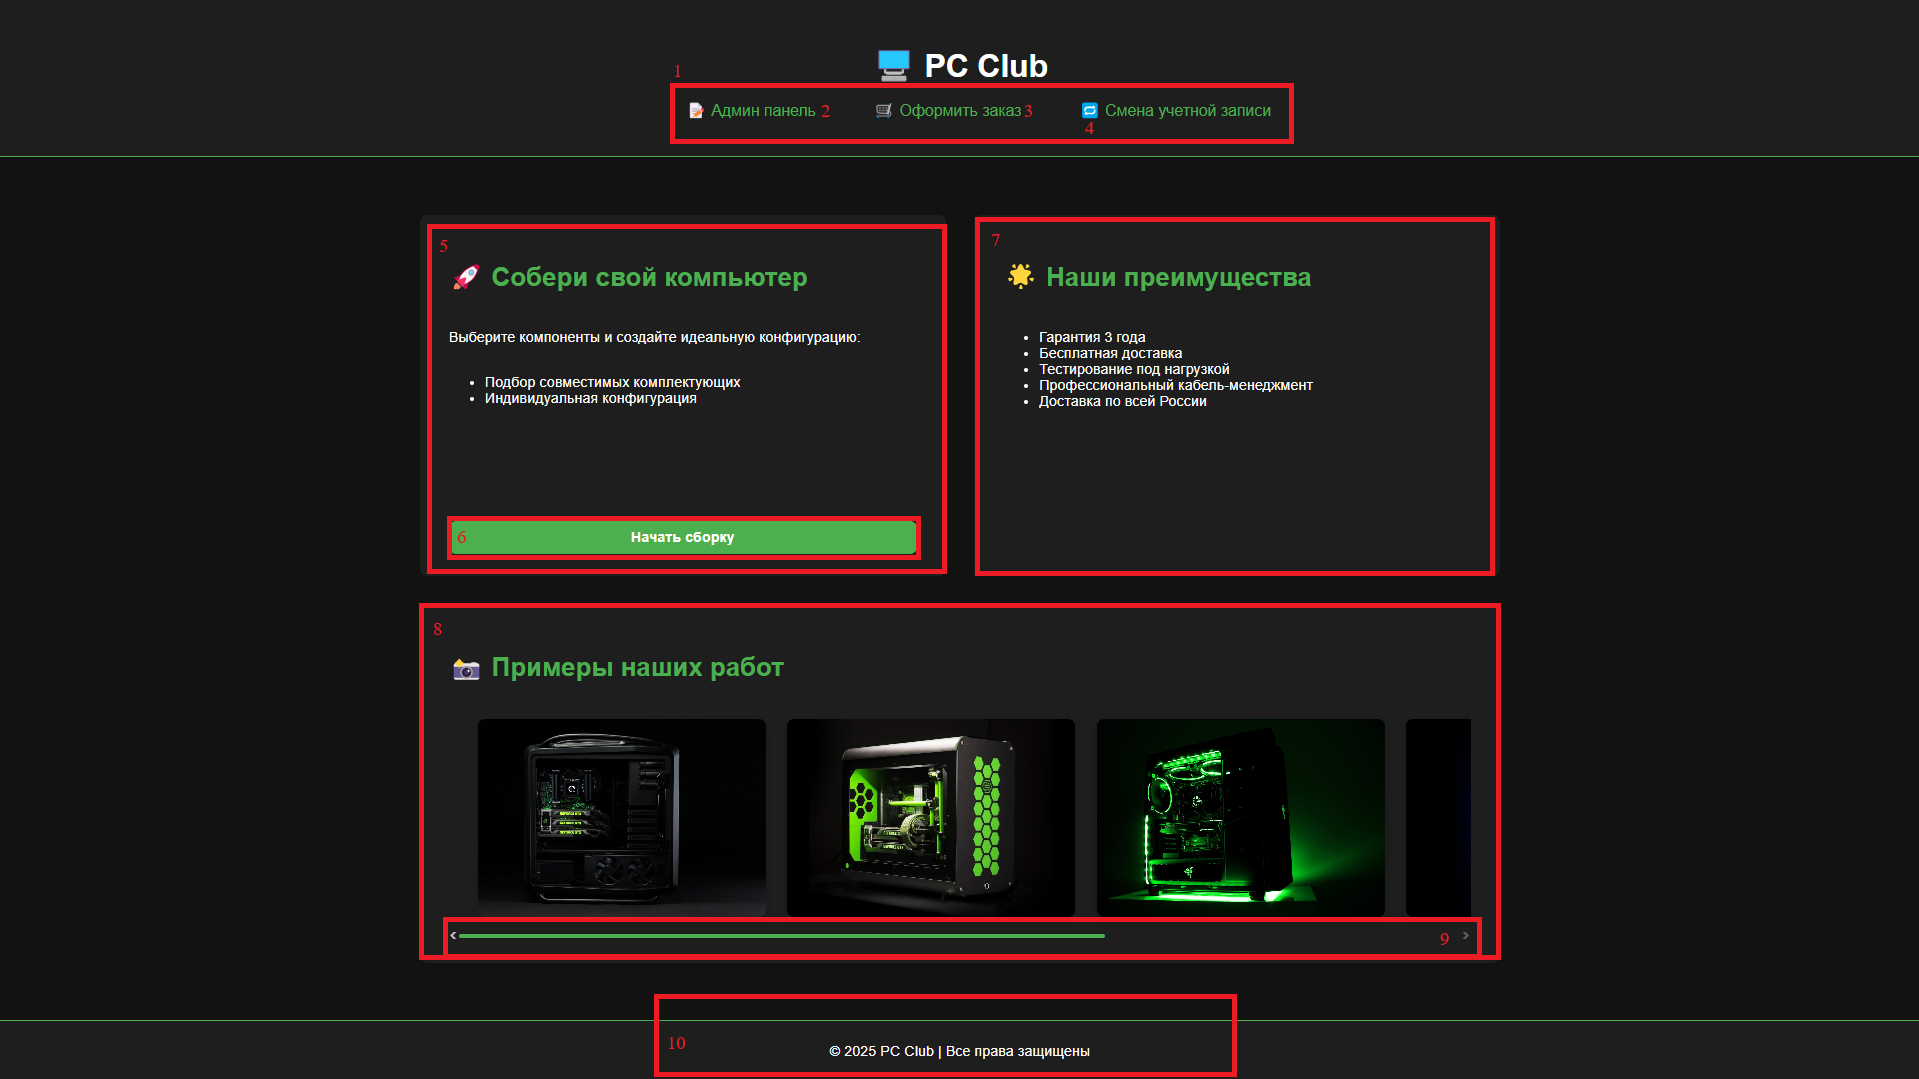
\includegraphics[width=1\linewidth]{index}}
\caption{Главная страница сайта.}
\label{index:image}
\end{figure}

\newpage 
На рисунке \ref{main:image} представлено меню оформления заказа,  в каждом поле можно вписать вручную или выбрать из выпадающего списка.
\begin{enumerate}
	\item Переход на страницу админ панели.
	\item Переход на главную страницу.
	\item Смена учетной записи.
	\item Простая форма ввода только чисел для цены.
	\item Форма ввода с календарем для вывода дат, проверяет на корректность.
	\item Простая форма ввода для адреса.
	\item Выбор из выпадающего списка.
	\item Выбор из выпадающего списка с возможностью ручного ввода.
	\item Кнопка собирает информацию с форм и отправляет в sql.
	\item Выпадающее меню.
	\item Поле ручного ввода/поиска по компонентам в sql.
	\item Кнопка развернуть.
	\item Виды комплектующих из sql.
	\item Сколько этих комплектующих осталось на складе.
\end{enumerate}

\begin{figure}[H]
\center{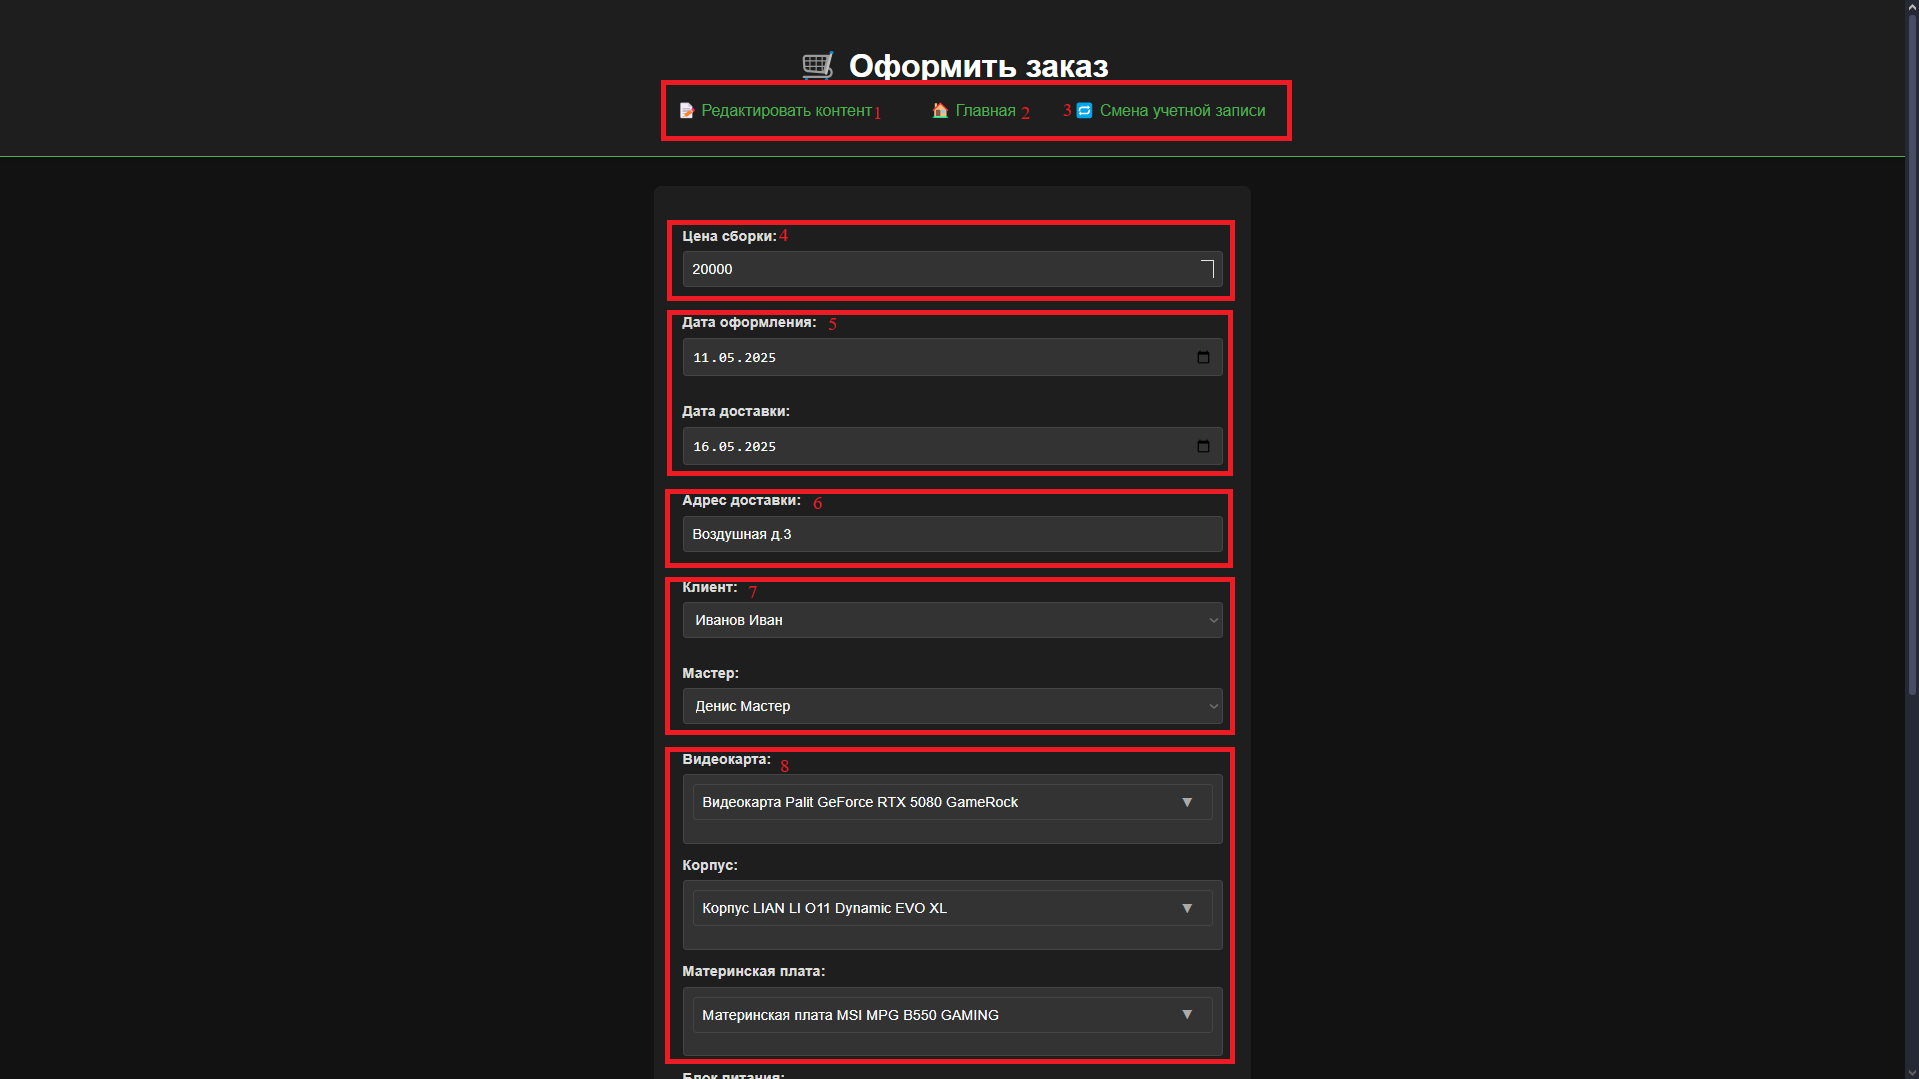
\includegraphics[width=0.9\linewidth]{order+fl}}
\center{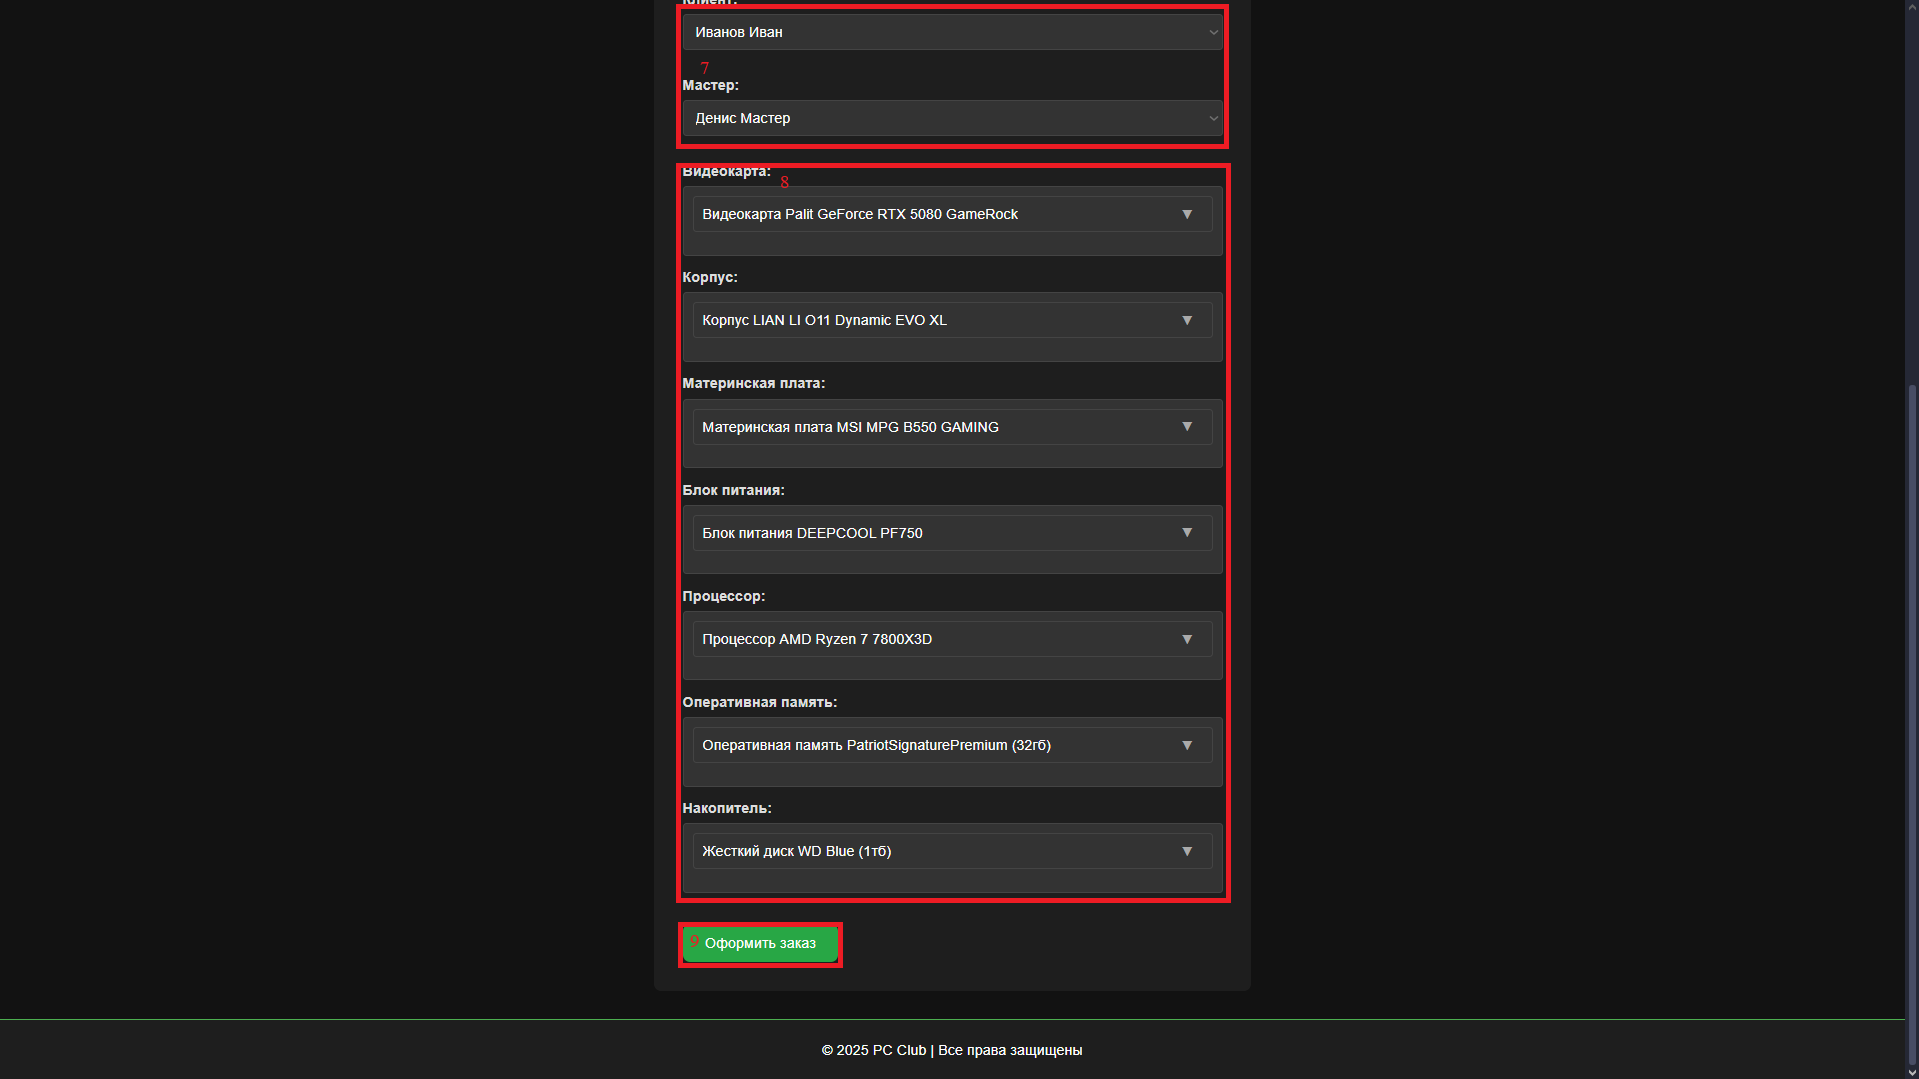
\includegraphics[width=0.9\linewidth]{order+fln}}
\center{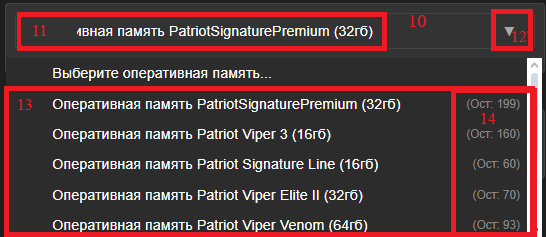
\includegraphics[width=0.75\linewidth]{chosenone}}
\caption{Страница оформления заказа и выпадающее меню компонента.}
\label{main:image}
\end{figure}

На рисунке \ref{login:image} меню для авторизации пользователей в системе, после авторизации под админской учетной записью можно получить доступ к админ панели, складу.
\begin{enumerate}
	\item Форма ввода логина.
	\item Форма ввода пароля.
	\item Кнопка сравнивает логин и хэш пароля с хранящимся в sql, при совпадении пропускает.
	\item Кнопка сохраняет логин и хэш пароля в sql.
	\item Вернуться на главную страницу.
\end{enumerate}
\begin{figure}[ht]
	\center{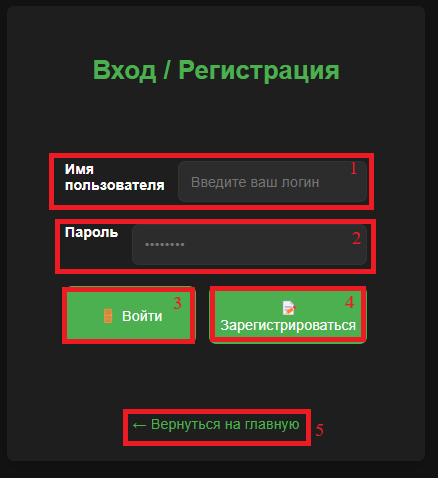
\includegraphics[width=0.25\linewidth]{login}}
	\caption{Разделы для каждого вида компонентов.}
	\label{login:image}
\end{figure}

На рисунке \ref{adminall:image} Панель администратора PC-Club позволяет полностью контролировать и редактировать информацию в sql.

\begin{enumerate}
	\item Панель навигации по сайту.
	\item Открыть меню выбора компонента.
	\item Ручной поиск по позициям и кнопка.
	\item Добавление новой записи в sql, через админ панель можно напрямую добавить новые компоненты в sql для их дальнейшего использования.
	\item Кнопка для редактирования, можно редактировать любую запись сделаную в таблицы sql.
	\item Кнопка для удаления, удалить любую запись из sql.
	\item Кнопка для экспорта данных таблицы заказа в файл.
	\item Заголовок таблицы, в нашем случае для заказов.
	\item Контент таблицы, хранимый и извлеченный из sql.
\end{enumerate}

\begin{figure}[ht]
\center{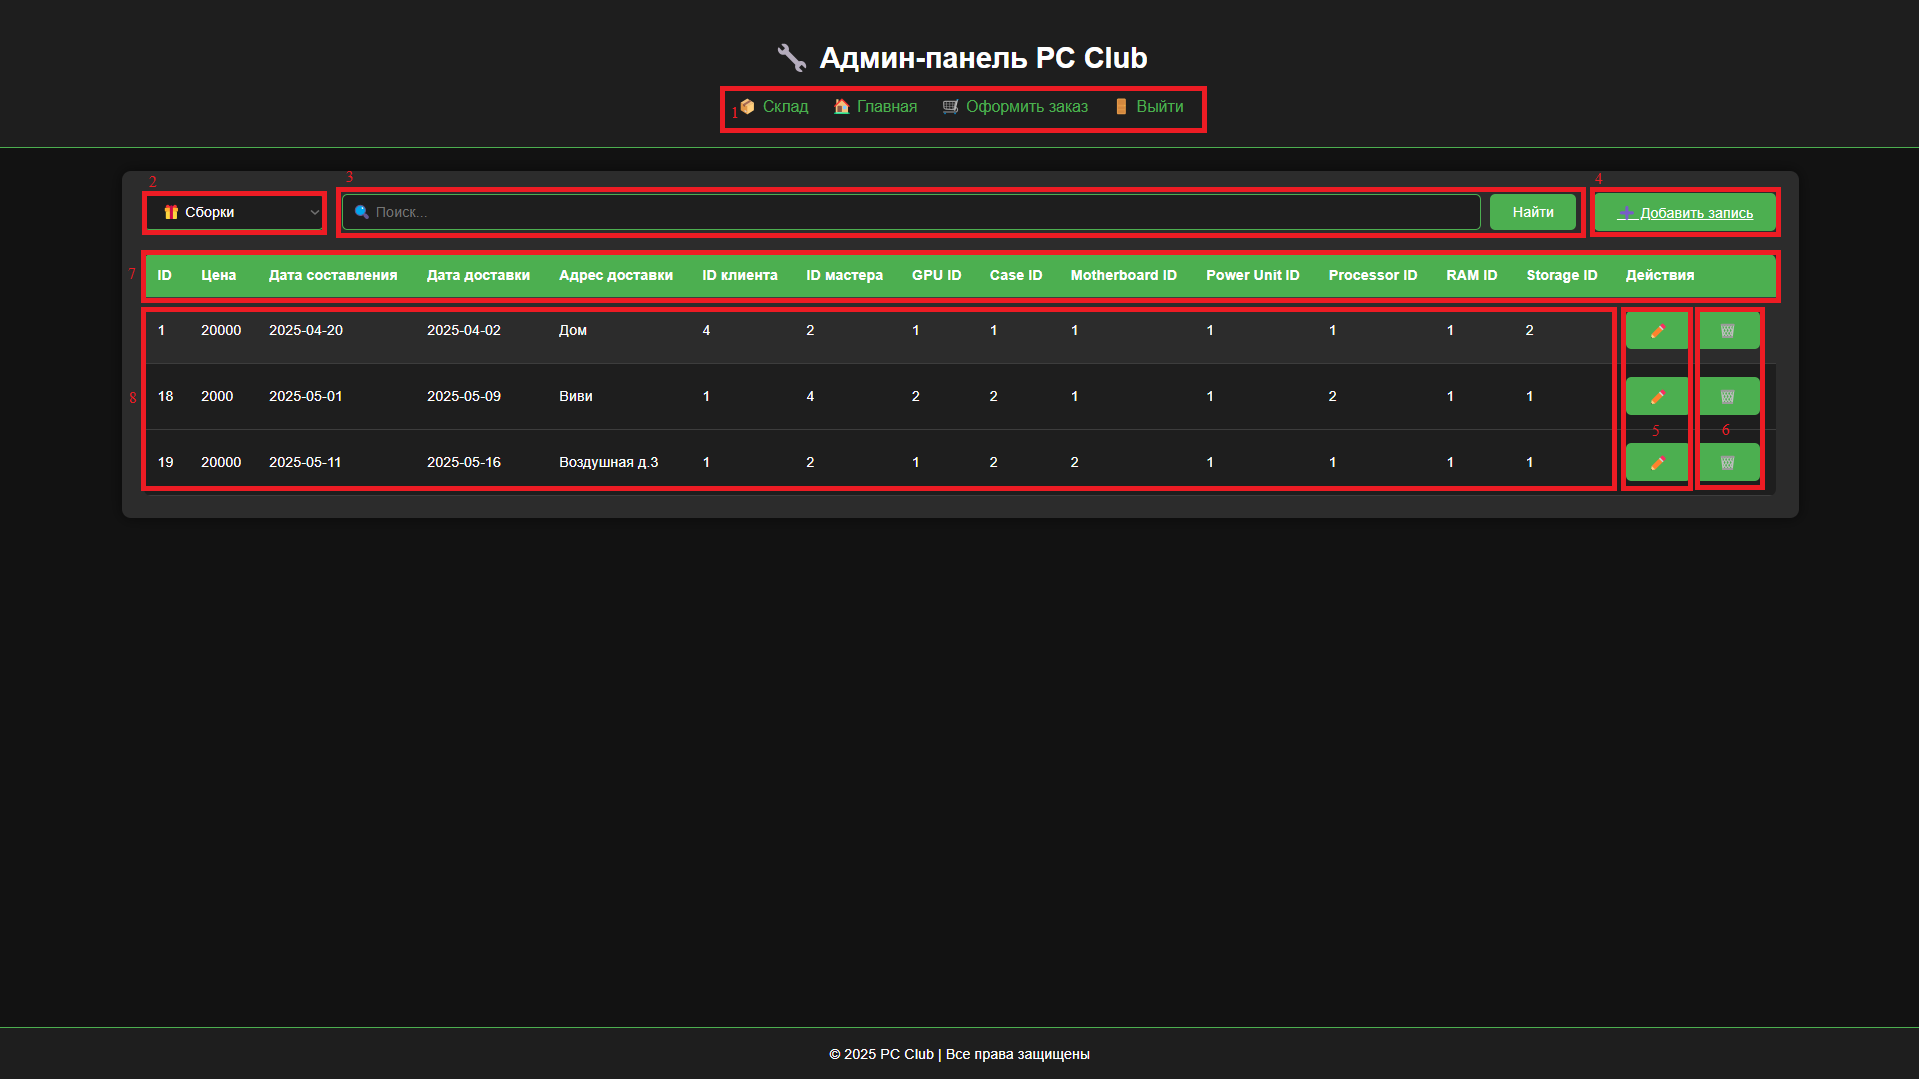
\includegraphics[width=1\linewidth]{adminall}}
\caption{Админ-панель PC-Club общий вид}
\label{adminall:image}
\end{figure}

На рисунке \ref{razdeli:image} меню выбора между типом компонентов в панели админа.

\begin{figure}[htbp]
\center{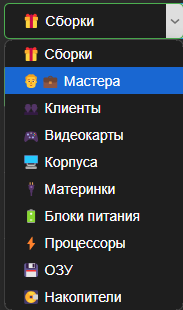
\includegraphics[width=0.25\linewidth]{razdeli}}
\caption{Разделы для каждого вида компонентов.}
\label{razdeli:image}
\end{figure}

На рисунке \ref{storedf:image} меню менеджмента склада для веб-приложения, здесь можно пополнять запасы недостающих комплектующих, потом применять их в заказах.

\begin{enumerate}
	\item Расширенная навигационная панель админа.
	\item Кнопка вызова меню выбора типа компонента.
	\item Ручной поиск по позициям и кнопка.
	\item Заголовок таблицы.
	\item Компонент из таблицы.
	\item Количество компонента на складе и поле для ввода нового значения.
	\item Кнопка для обновления значения.
\end{enumerate}

\begin{figure}[ht]
	\center{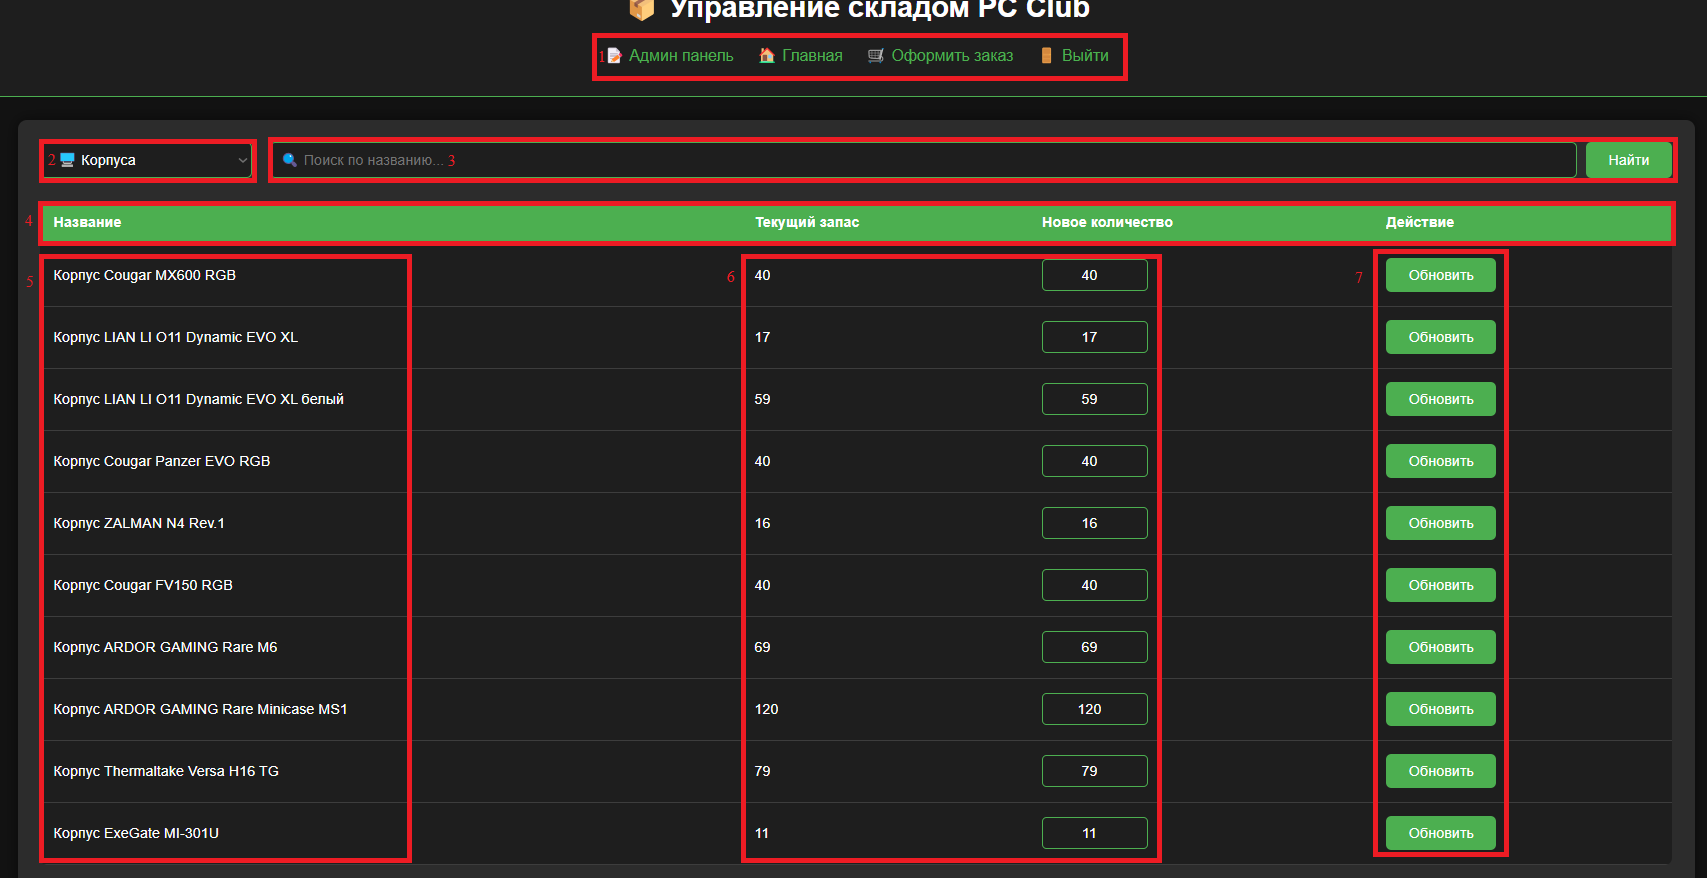
\includegraphics[width=1\linewidth]{storedf}}
	\caption{Страничка склада корпусов в качестве примера.}
	\label{storedf:image}
\end{figure}
\clearpage

\subsection{Тестирование программной системы}
Целью данного тестирования является проверка функциональности, надежности и производительности программно-информационной системы для управления сервис-центром.
Системное тестирование позволяет выявить и устранить ошибки, а также оценить соответствие системы предъявленным требованиям.

Все тестовые сценарии должны быть выполнены успешно без критических ошибок. Система должна обеспечивать стабильную работу и удобство использования в рамках установленных бизнес-процессов. Результаты тестирования будут использованы для повышения качества и надежности программного продукта.

\textbf{1) Запуск системы}

Описание: Система должна запускаться без ошибок и отображать главное окно интерфейса.

\begin{figure}[ht]
	\center{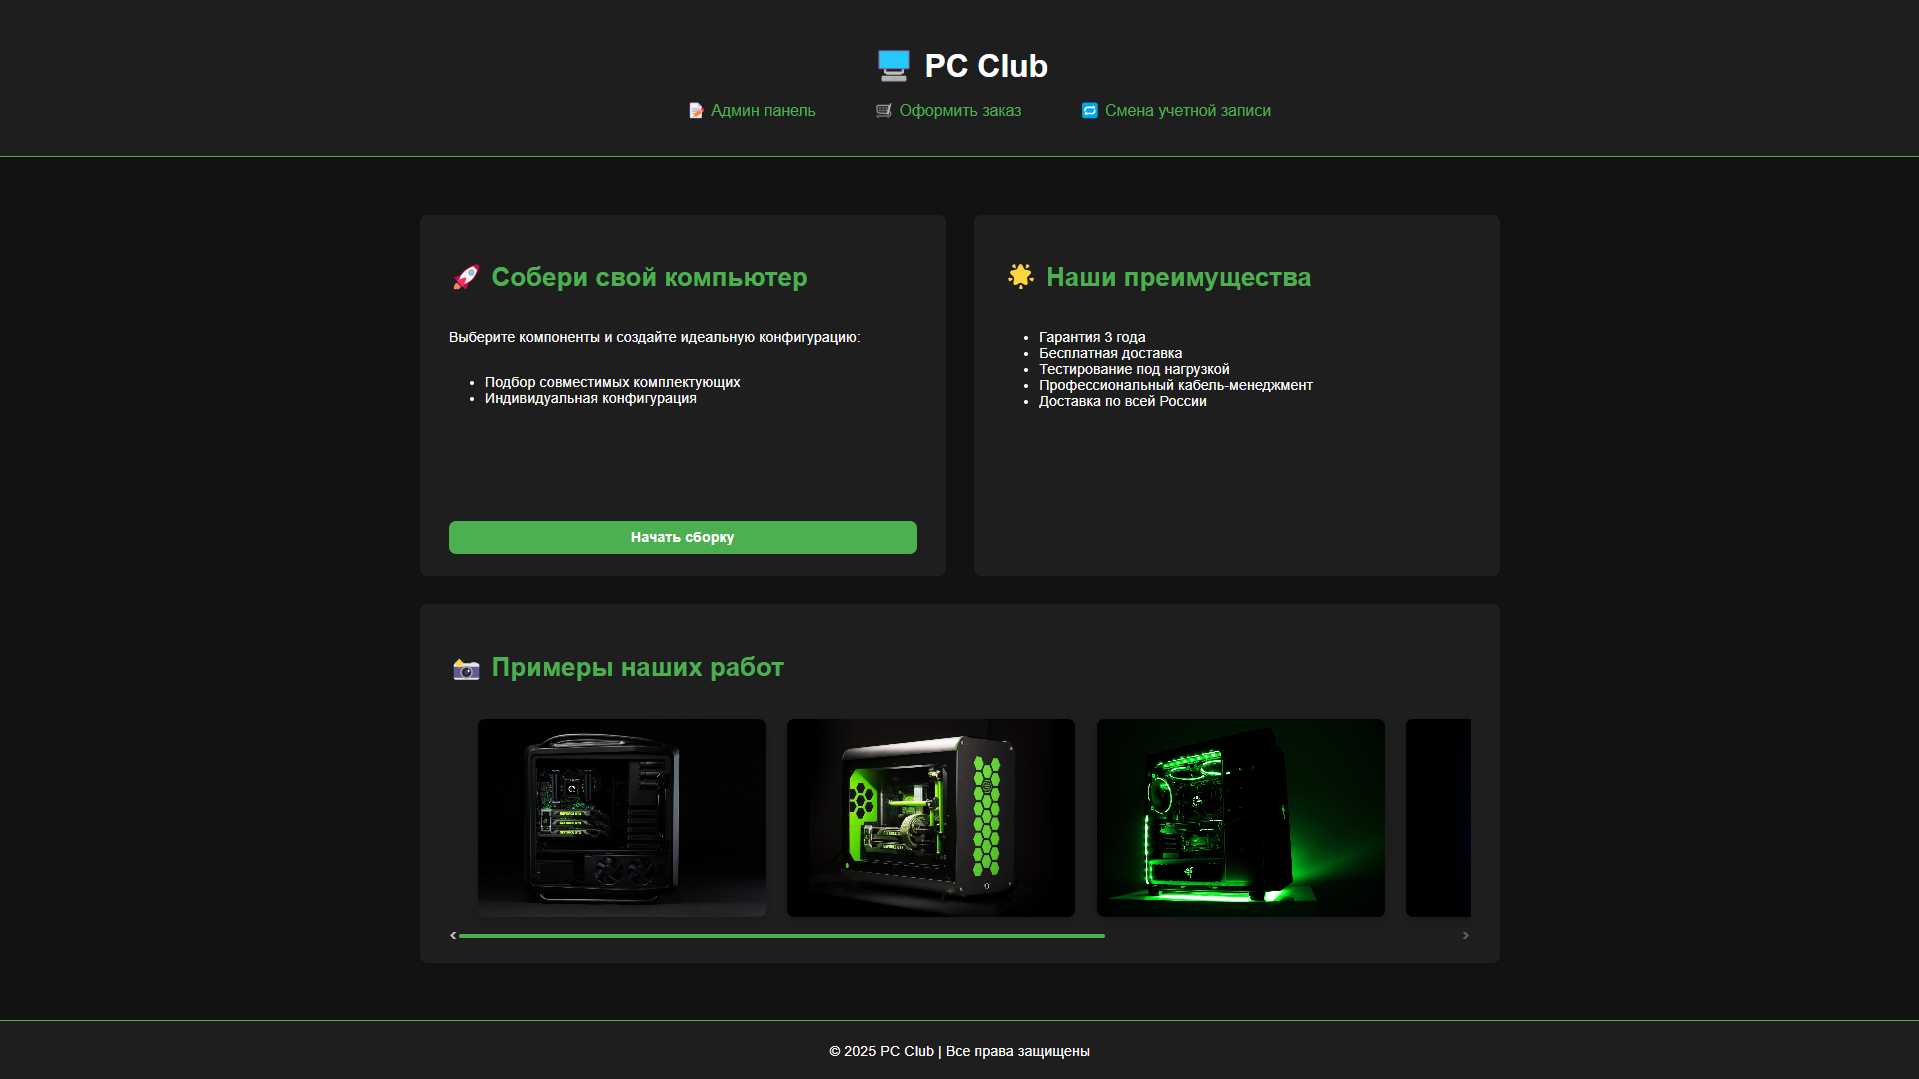
\includegraphics[width=1\linewidth]{index0}}
	\caption{Главная страница.}
	\label{storedf:index0}
\end{figure}

\newpage

\textbf{2) Регистрация пользователя}

Описание: Пользователь должен иметь возможность создать новую учетную запись в системе.
Ожидаемый результат:  При вводе имени пользователя и пароля, нажатии на кнопку "Регистрация" пользователь создает новую запись в SQL.

\begin{figure}[ht]
	\center{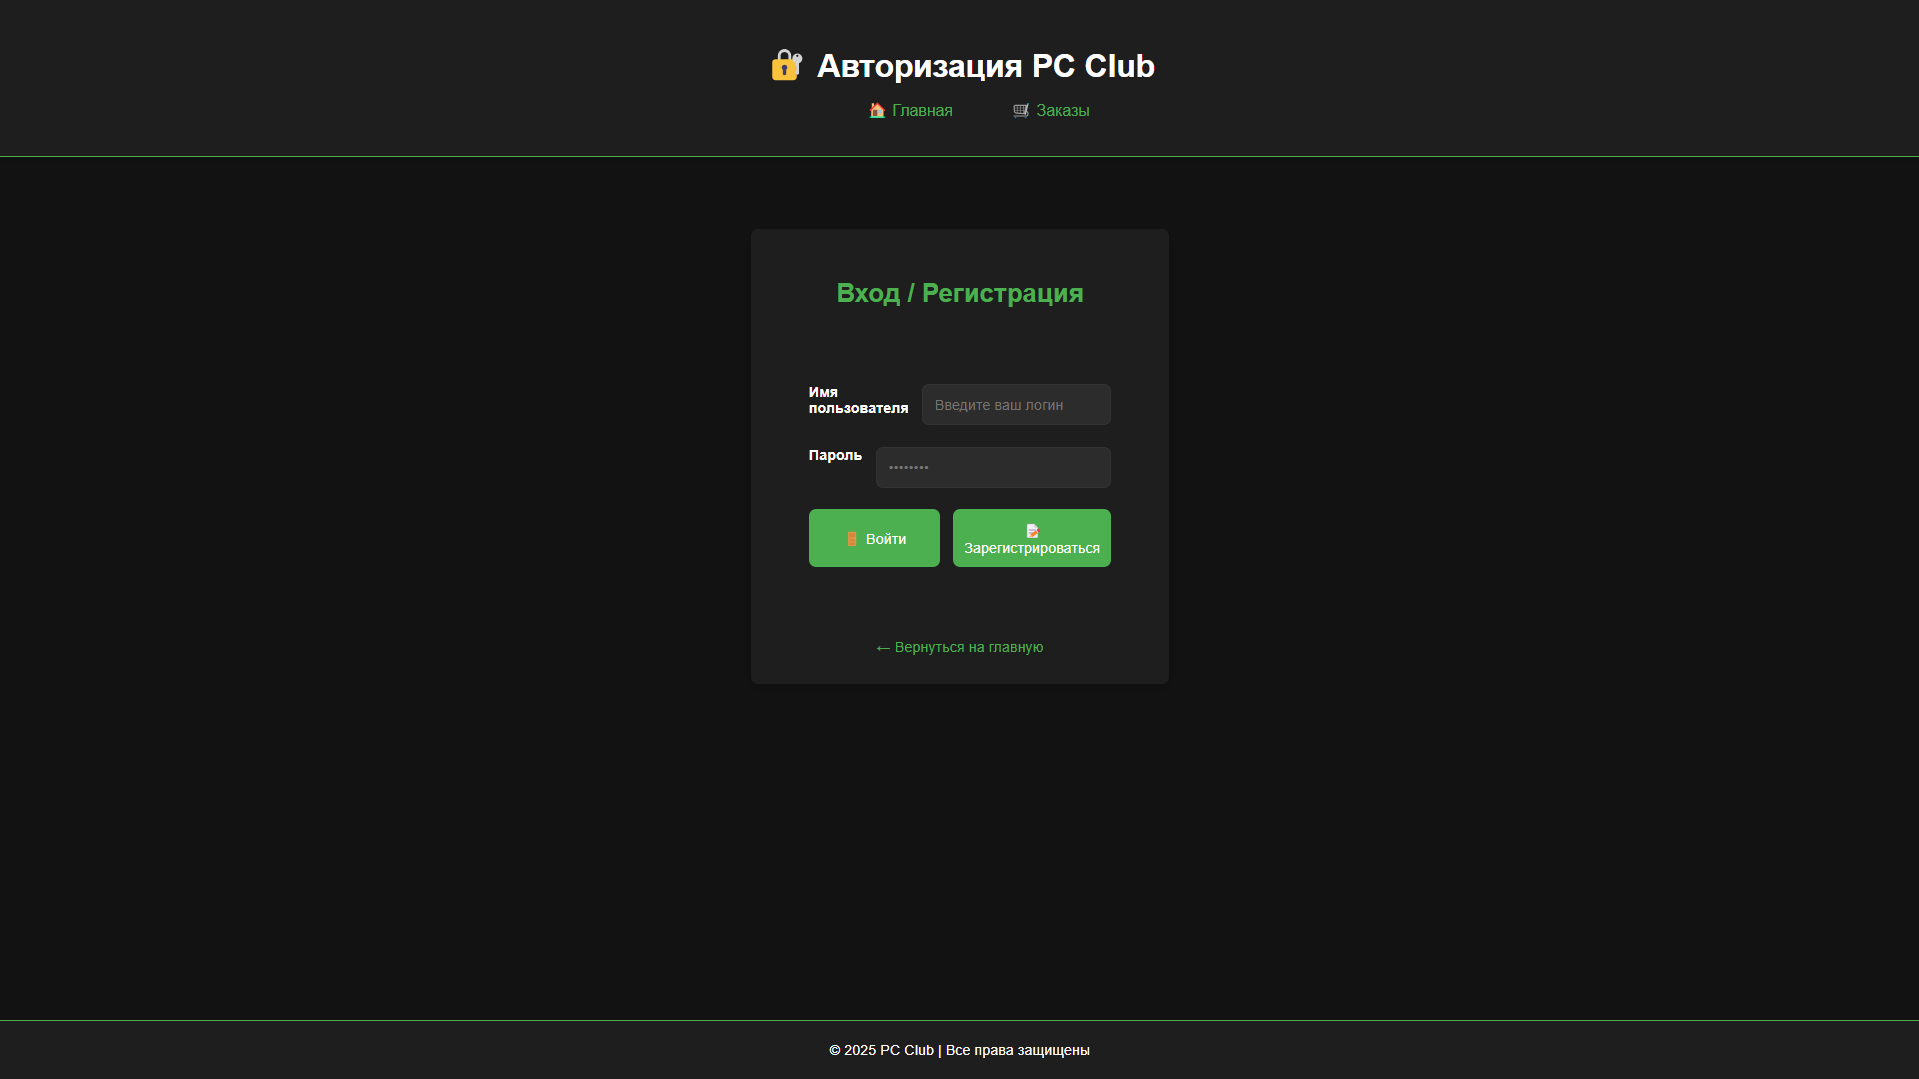
\includegraphics[width=0.9\linewidth]{login0}}
	\caption{Страница логин.}
	\label{storedf:login0}
\end{figure}

\begin{figure}[ht]
	\center{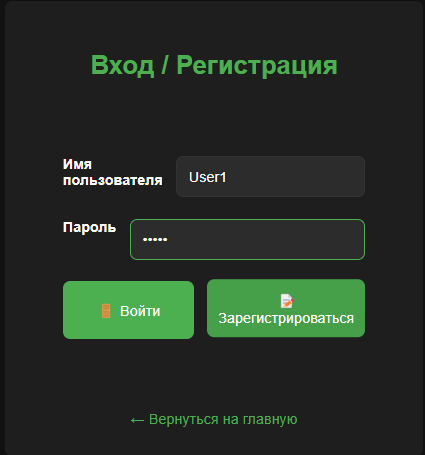
\includegraphics[width=0.5\linewidth]{loginus}}
	\caption{Регистрация.}
	\label{storedf:loginus}
\end{figure}

\begin{figure}[ht]
	\center{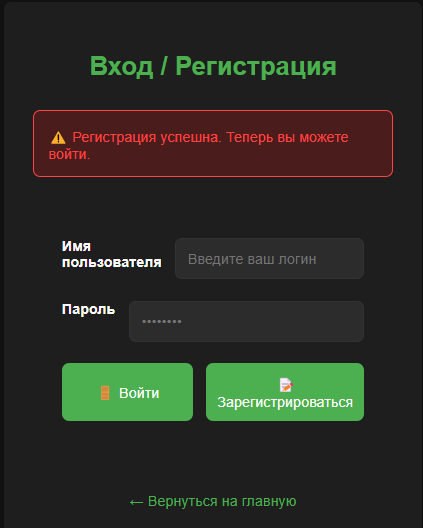
\includegraphics[width=0.5\linewidth]{loginc}}
	\caption{Результат регистрации.}
	\label{storedf:loginc}
\end{figure}

Новая запись добавляется в SQL таблицу users, без прав администратора. Пароль хэшируется для безопасного хранения данных пользователей.

\begin{figure}[ht]
	\center{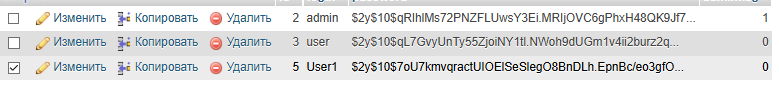
\includegraphics[width=1\linewidth]{login1}}
	\caption{Результат регистрации в SQL.}
	\label{storedf:login1}
\end{figure}

\textbf{2) Авторизация пользователя}

Описание: Пользователь должен иметь возможность войти в свою учетную запись используя корректные имя пользователя и пароль.
Ожидаемый результат: Пользователь входит в свою учетную запись и получает доступ к своим функциям.

\begin{figure}[ht]
	\center{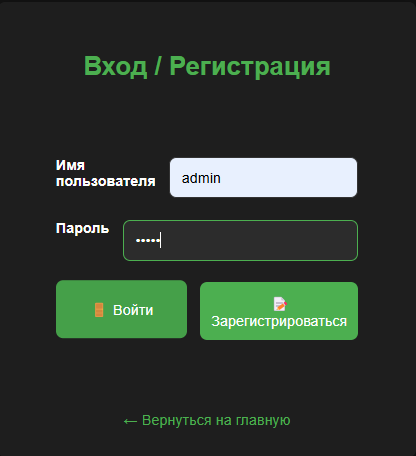
\includegraphics[width=0.6\linewidth]{loginad}}
	\caption{Окно авторизации.}
	\label{storedf:loginad}
\end{figure}

\begin{figure}[ht]
	\center{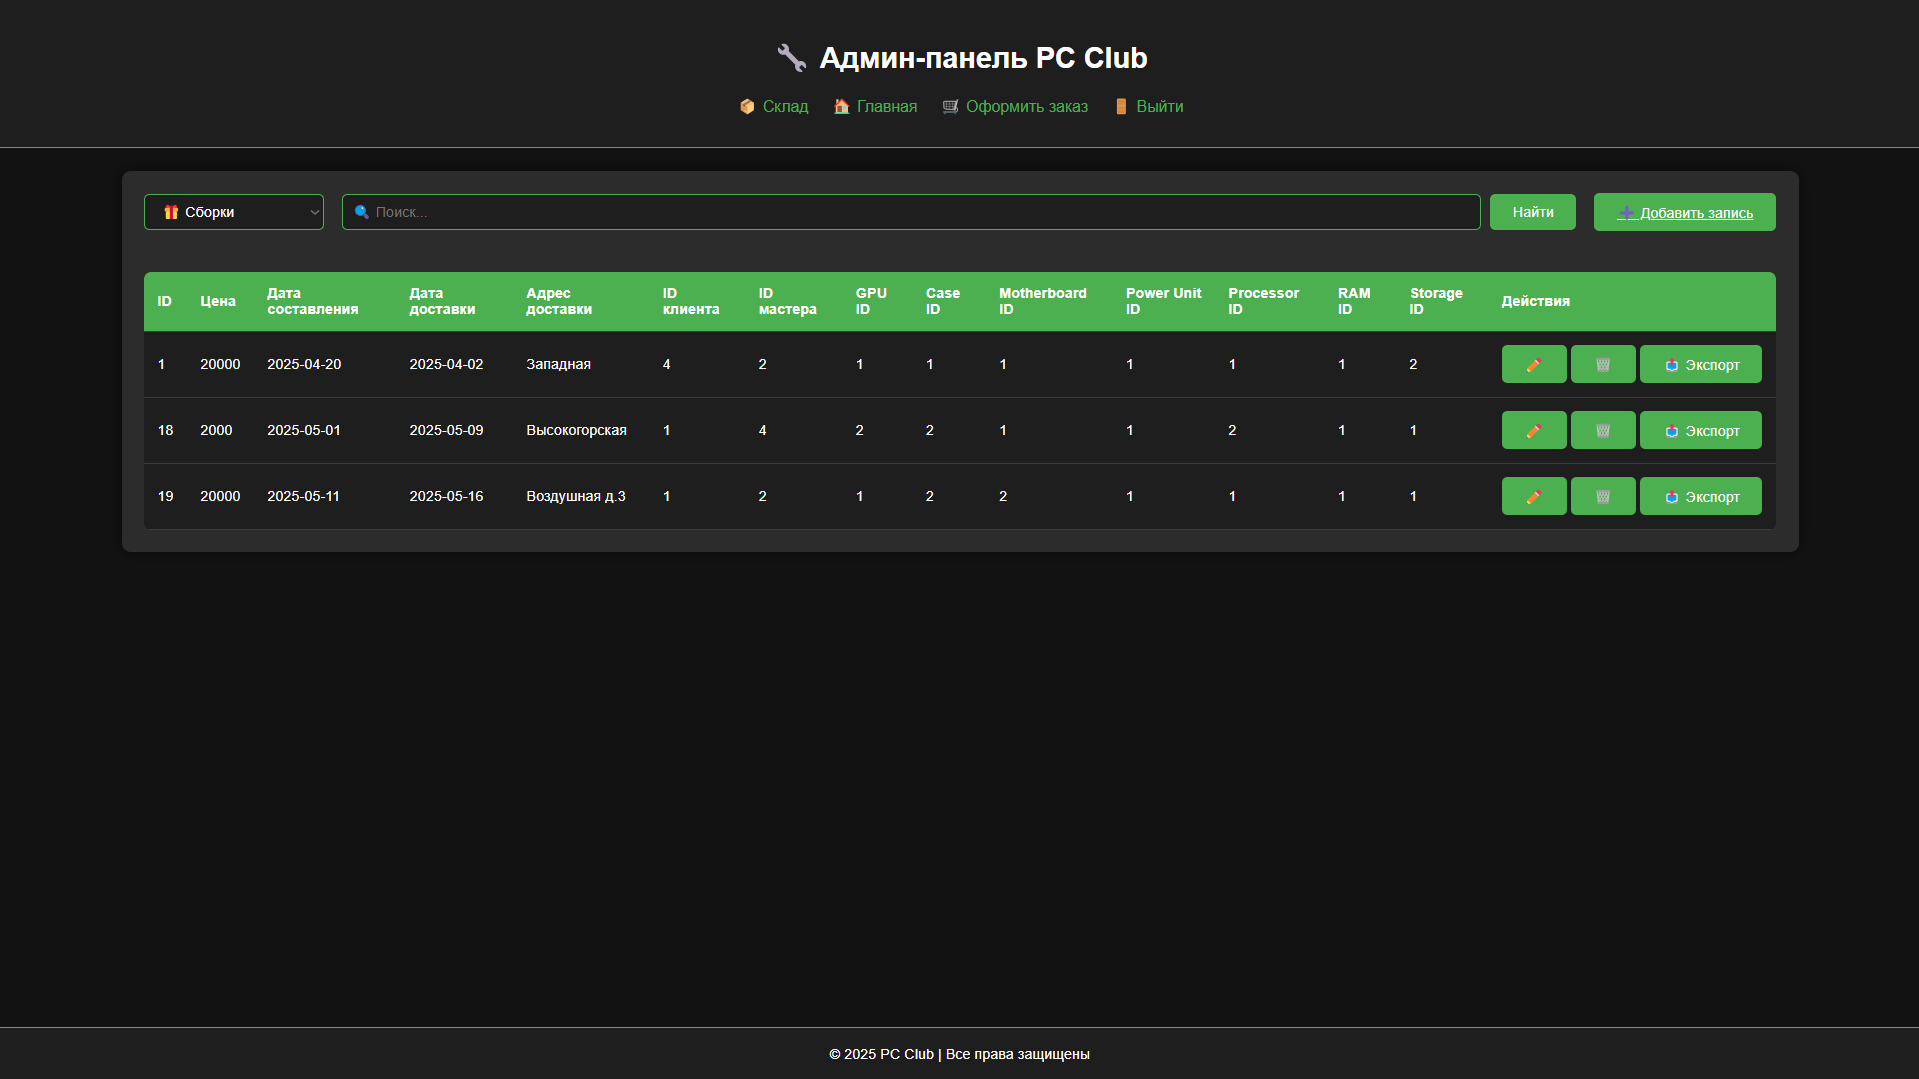
\includegraphics[width=0.9\linewidth]{panel0}}
	\caption{Результат авторизации пользователя.}
	\label{storedf:panel0}
\end{figure}

\newpage

\textbf{3) Оформление заказа}

Описание: Пользователь должен иметь возможность создать новый заказ в системе.
Ожидаемый результат:  При вводе всех данных корректно отправляет новый заказ в систему.

\begin{figure}[ht]
	\center{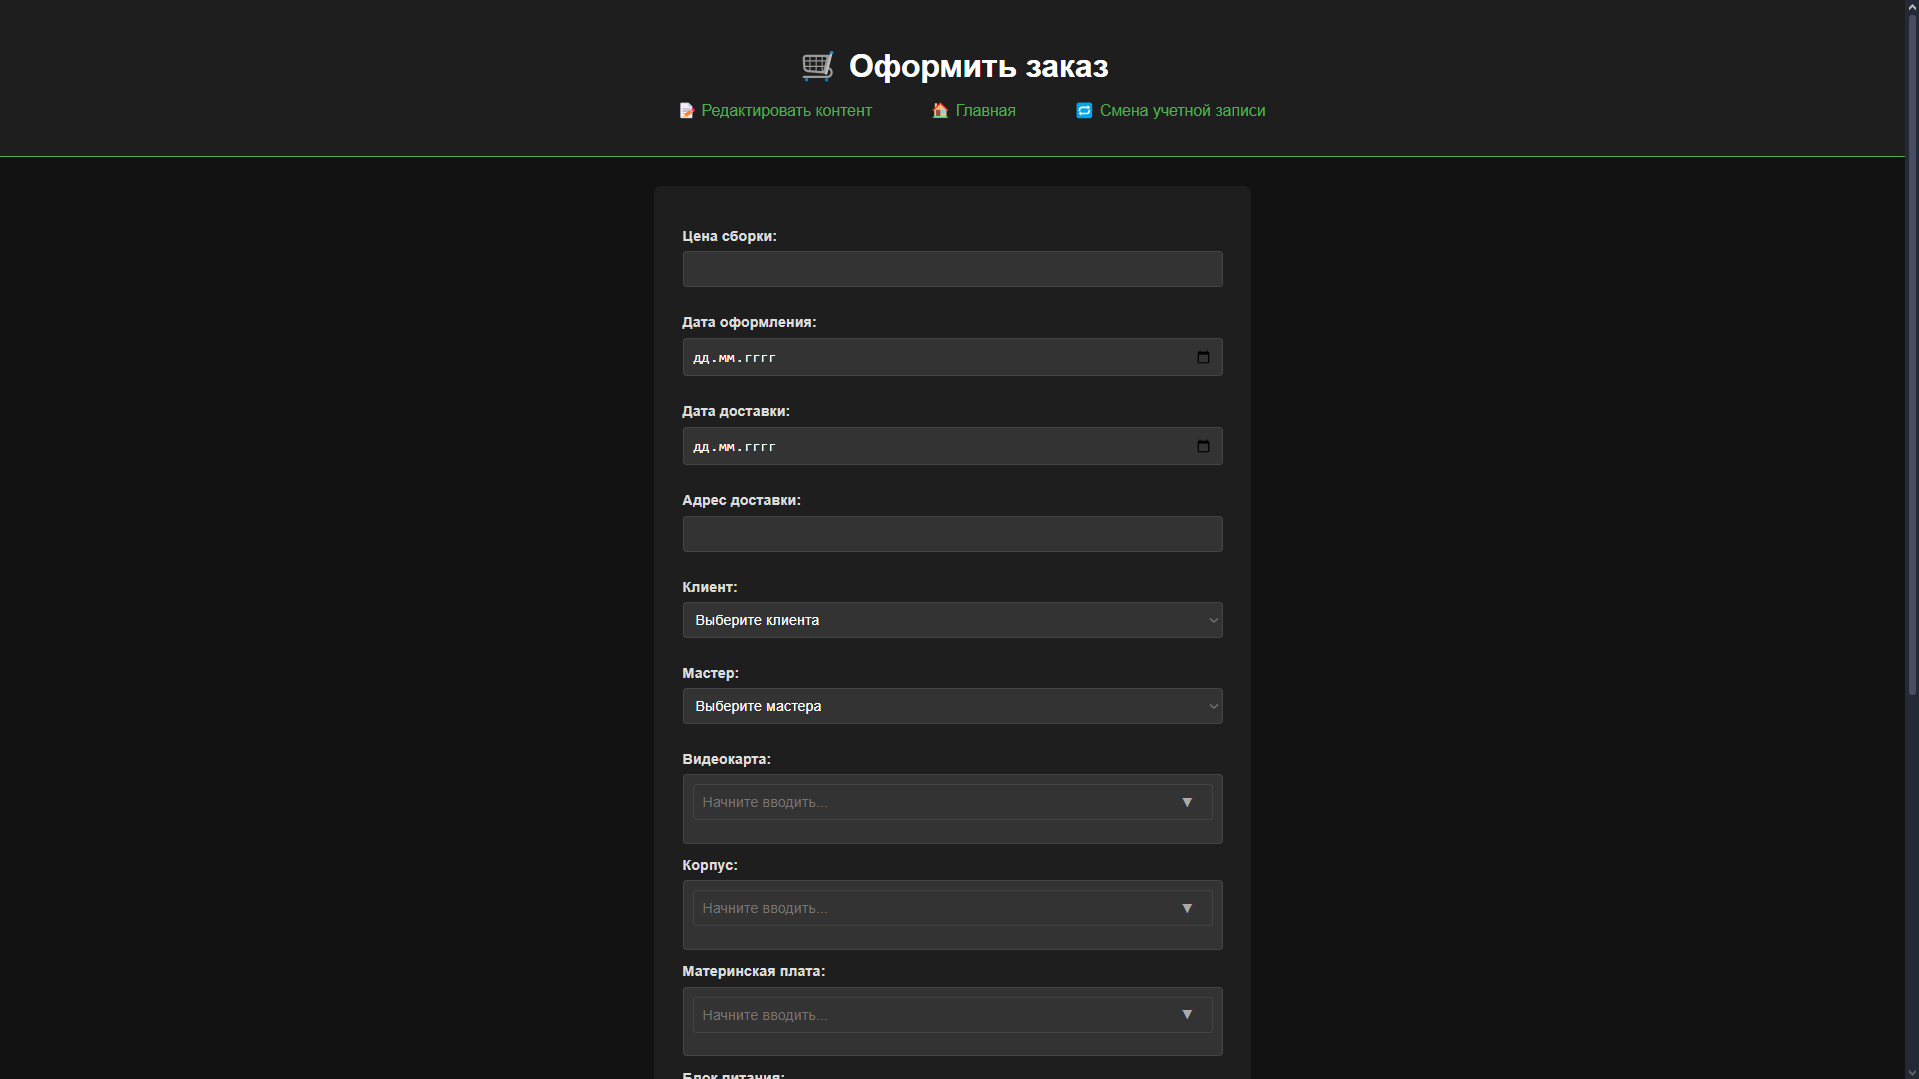
\includegraphics[width=0.9\linewidth]{form0}}
	\caption{Окно оформления заказа.}
	\label{storedf:form0}
\end{figure}

\begin{figure}[ht]
	\center{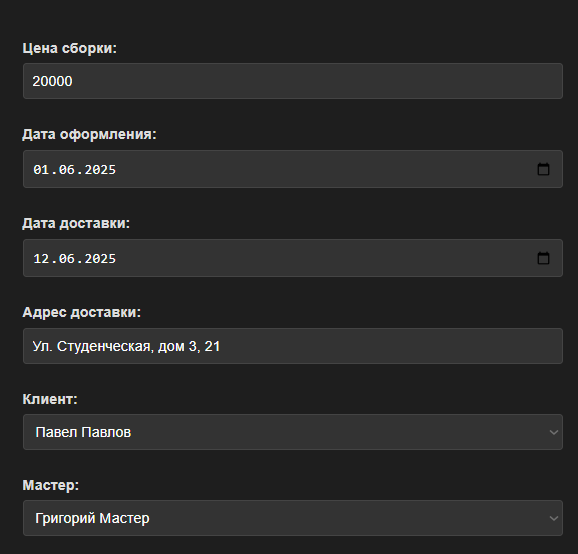
\includegraphics[width=0.5\linewidth]{form1}}
	\caption{Ввод данных заказа.}
	\label{storedf:form1}
\end{figure}

\begin{figure}[ht]
	\center{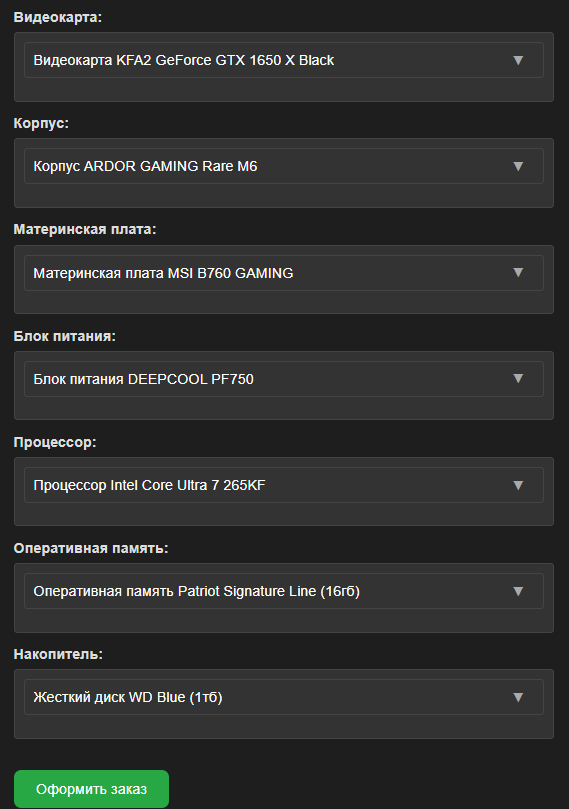
\includegraphics[width=0.5\linewidth]{form2}}
	\caption{Ввод технических данных компонентов заказа.}
	\label{storedf:form2}
\end{figure}

\begin{figure}[ht]
	\center{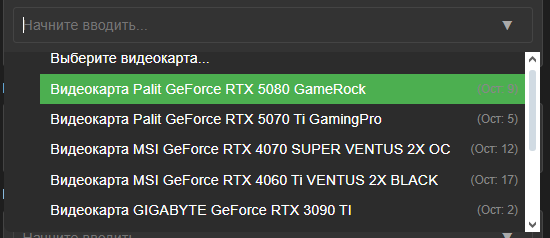
\includegraphics[width=0.4\linewidth]{formsearch0}}
	\caption{Селектор компонентов.}
	\label{storedf:formsearch0}
\end{figure}

\begin{figure}[ht]
	\center{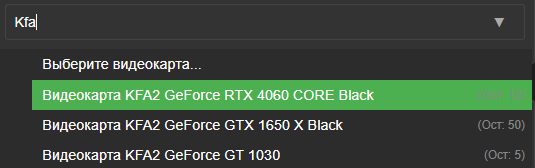
\includegraphics[width=0.4\linewidth]{formsearch1}}
	\caption{Результат поиска в селекторе.}
	\label{storedf:formsearch1}
\end{figure}

\begin{figure}[ht]
	\center{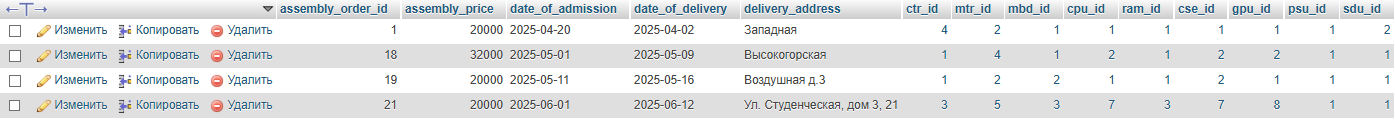
\includegraphics[width=0.9\linewidth]{formgg1}}
	\caption{Результат оформления заказа в SQL.}
	\label{storedf:formgg1}
\end{figure}
\clearpage

\textbf{4) Отображение панели администратора}

Описание: Пользователь авторизован как администратор, панель администратора должна отображаться без ошибок. 

\begin{figure}[ht]
	\center{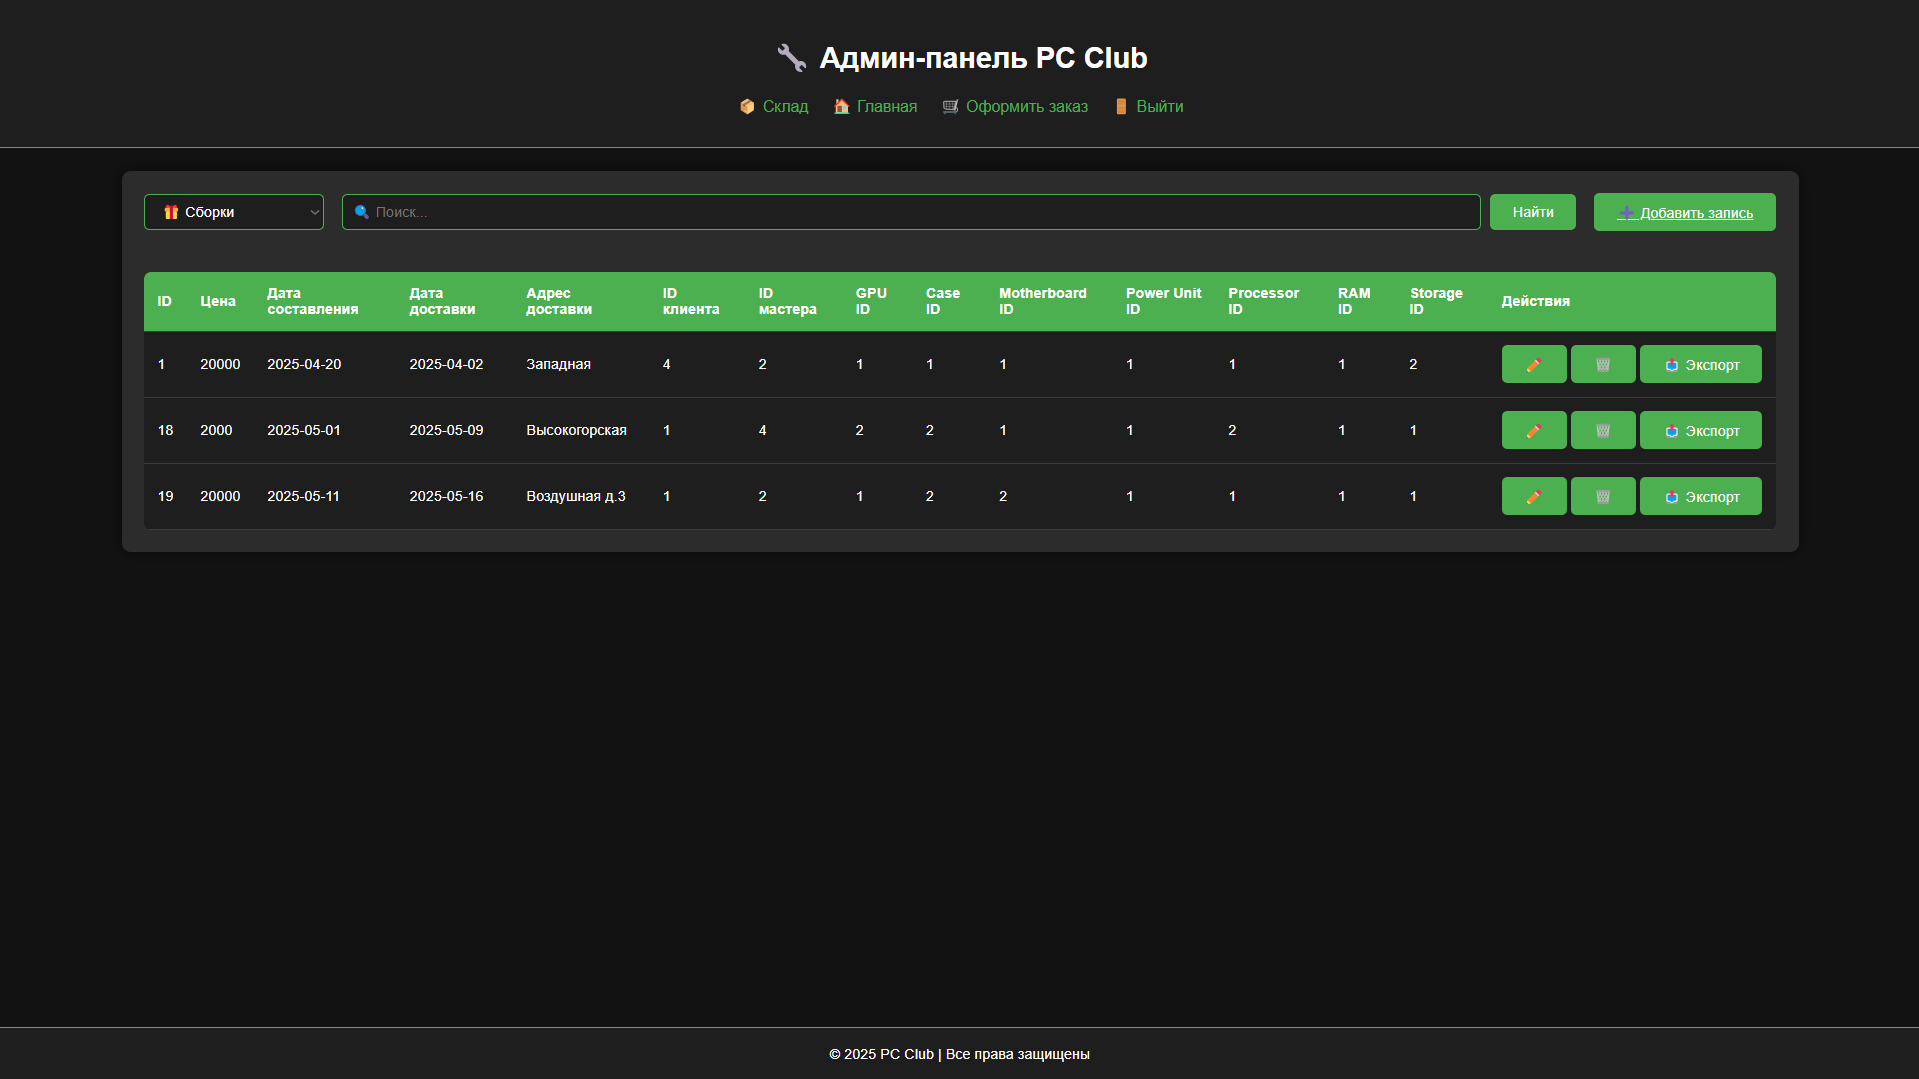
\includegraphics[width=0.9\linewidth]{panel0}}
	\caption{Отображение рабочей панели администратора.}
	\label{storedf:panel0_}
\end{figure}

\textbf{5) Редактирование данных записи}
\begin{enumerate}
\item Пользователь нажимает на кнопку "карандаш".
\item Меняет данные в заказе.
\item Сохраняет изменения.
\end{enumerate}

\begin{figure}[ht]
	\center{
\includegraphics[width=0.9\linewidth]{edit1}}
	\caption{Результат редактирования.}
	\label{storedf:edit1}
\end{figure}

\begin{figure}[ht]
	\center{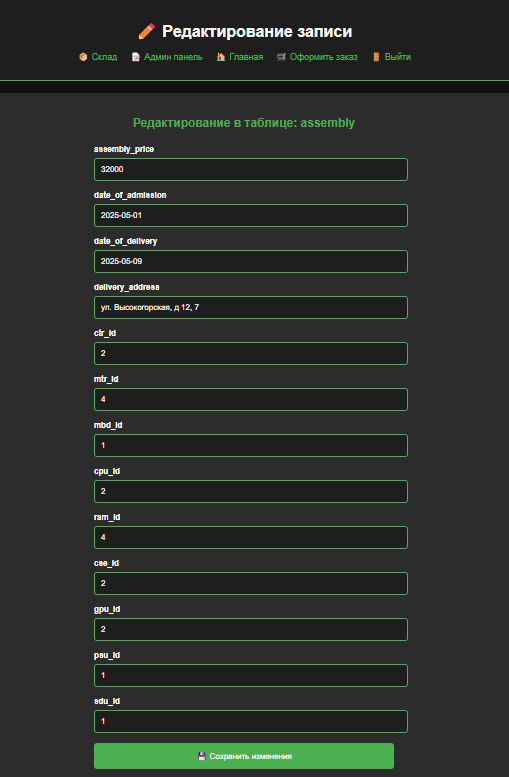
\includegraphics[width=0.8\linewidth]{edit0}}
	\caption{Интерфейс редактирования.}
	\label{stored:edit0}
\end{figure}

\clearpage

\textbf{6) Добавление новой записи}
\begin{enumerate}
	\item Пользователь нажимает на кнопку "добавить".
	\item Заполняет форму.
	\item Сохраняет запись.
\end{enumerate}

\begin{figure}[ht]
	\center{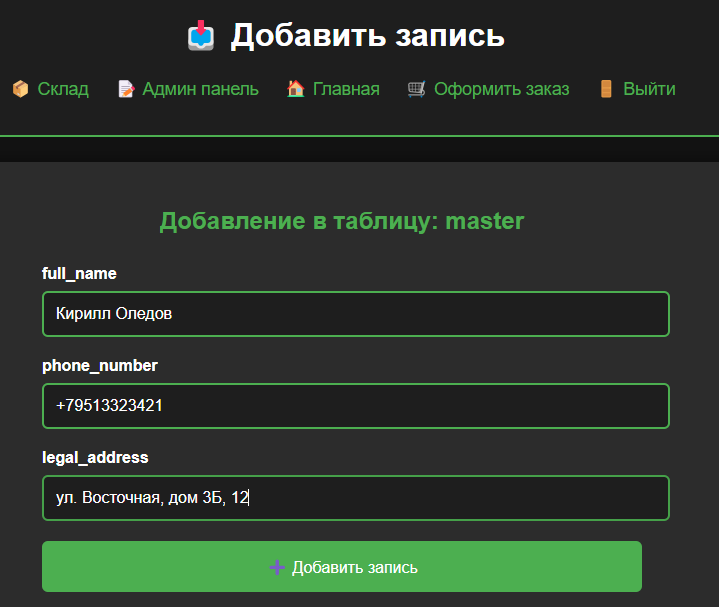
\includegraphics[width=0.7\linewidth]{addone}}
	\caption{Добавление новой записи.}
	\label{stored:addone}
\end{figure}

\begin{figure}[ht]
	\center{
\includegraphics[width=0.8\linewidth]{addone1}}
	\caption{Новая запись в системе.}
	\label{stored:addone1}
\end{figure}

\textbf{7) Удаление записи}
\begin{enumerate}
	\item Пользователь нажимает на кнопку "удалить".
	\item Подтверждает удаление.
\end{enumerate}

\begin{figure}[ht]
	\center{
\includegraphics[width=0.5\linewidth]{delete}}
	\caption{Новая запись в системе.}
	\label{stored:delete}
\end{figure}

\clearpage

\textbf{8) Экспорт заказа в файл}
\begin{enumerate}
	\item Пользователь нажимает на кнопку "экспорт".
	\item Пользователь получает файл с информацией о заказе.
\end{enumerate}

\begin{figure}[ht]
	\center{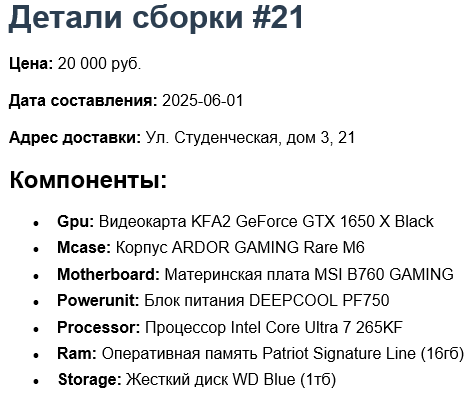
\includegraphics[width=1\linewidth]{docdoc}}
	\caption{Сгенерированный .doc файл, содержит информацию о заказе.}
	\label{stored:docdoc}
\end{figure}

\textbf{9) Редактирование количества компонентов на складе}
Описание: Пользователь должен иметь возможность редактировать количество компонентов на складе.
Ожидаемый результат: Редактирует значение stock у требуемых компонентов.

\begin{figure}[ht]
	\center{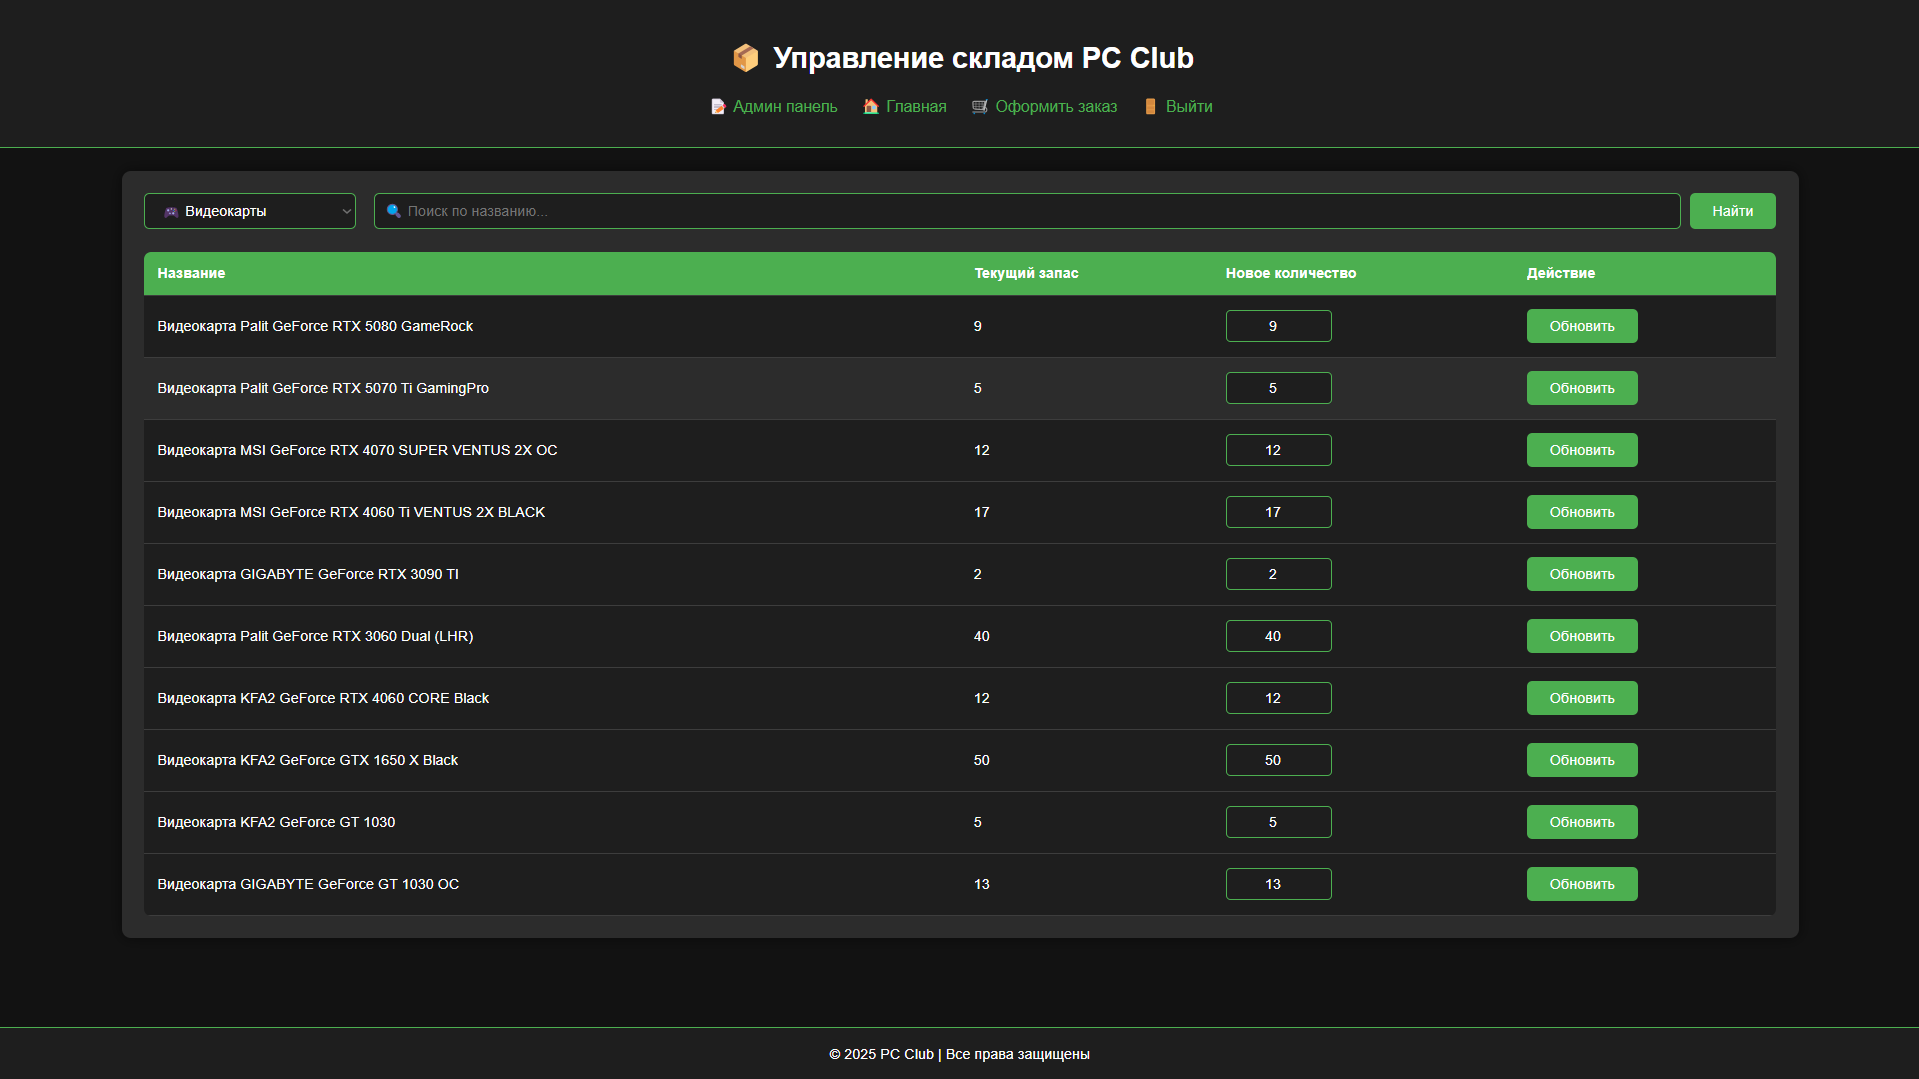
\includegraphics[width=1\linewidth]{warehouse0}}
	\caption{Окно с количеством компонентов на складе.}
	\label{stored:warehouse0}
\end{figure}

\begin{figure}[ht]
	\center{
\includegraphics[width=1\linewidth]{stock0}}
	\caption{Добавляем новое количество компонента.}
	\label{stored:stock0}
\end{figure}

\begin{figure}[ht]
	\center{
\includegraphics[width=1\linewidth]{stock1}}
	\caption{Уведомление об успехе.}
	\label{stored:stock1}
\end{figure}

\begin{figure}[ht]
	\center{
\includegraphics[width=1\linewidth]{stock2}}
	\caption{Обновленное количество компонента.}
	\label{stored:stock2}
\end{figure}

\clearpage